\section{Гетероструктура}
\begin{definition}{\textsc{Гетероструктура}}
	Полупроводниковая структура с несколькими гетеропереходами (ГП). Возможность изменять на границах ГП ширину запрещённой зоны позволяет эффективно управлять движением носителей заряда.
\end{definition}

\begin{definition}{\textsc{Гетеропереход}}
	Контакт двух различных по химическому составу монокристаллических или аморфных полупроводников.
\end{definition}

ГП может образоваться между полупроводниками с абсолютно одинаковыми постоянными решетки, образующими монолитный, однородный в контакте, кристалл.
\begin{enumerate}
	\item $GaAs$--$AlAs$;
	\item $GaN$--$AlN$;
	\item $GaSb$--$AlSb$--$InAs$;
	\item $GaAs$--$Ge$.
\end{enumerate}
Чаще всего в качестве материалов для ГС используются $GaAs$ и твердый раствор $Al_{x}Ga_{1−x}As$.

\subsection{Зонная диаграмма}
Наряду с плавным изменением энергий краев зоны проводимости и валентной зоны, которое, как и в обычном $p$--$n$--переходе, определяется разностью работ выхода контактирующих полупроводников и длиной экранирования объемного заряда, на переходе имеются разные скачки в изменении энергии.

Согласно модели Андерсона, скачок в изменении энергии для зоны проводимости:
\begin{gather}
	\Delta \varepsilon_{c} = \chi_{1} - \chi_{2};\\
	\Delta \varepsilon_{v} = \Delta \varepsilon_{g} - \Delta \varepsilon_{c};
\end{gather}

\begin{figure}[h]
  \centering
  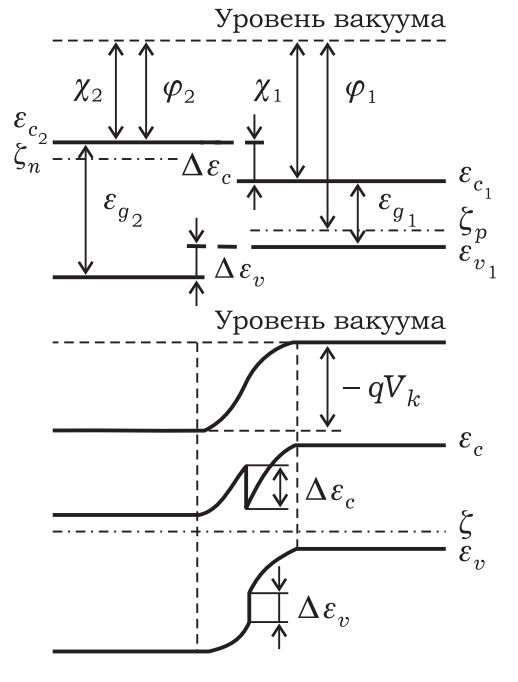
\includegraphics[width=.5\linewidth]{assets/profile}
  \caption{Зонная диаграмма перехода между электронными и дырочными полупроводниками с разной шириной запрещенной зоны}
  \label{img:2.0.0}
\end{figure}

\subsection{Гетероструктуры на основе $Al_{x}Ga_{1−x}As$}
Рассмотрим основные характеристики $Al_{x}Ga_{1−x}As$.

\begin{center}
  \begin{longtable}{|c|c|}
    \caption{Основные параметры $Al_{x}Ga_{1−x}As$}
    \label{tab:2.0.0}
    \\ \hline
    Параметр & $Al_{x}Ga_{1−x}As$ \\
    \hline \endfirsthead
    \subcaption{Продолжение таблицы~\ref{tab:2.0.0}}
    \\ \hline \endhead
    \hline \subcaption{Продолжение на след. стр.}
    \endfoot
    \hline \endlastfoot
	Кристаллическая структура& Типа цинковой обманки \\ \hline
	Постоянная решетки $a[nm]$  & $0.56533+0.00078x$ \\ \hline
	$E_{g}^{\Gamma}[eV],\, x < 0.45$    & $0.56533+0.00078x$ \\ \hline
	$E_{g}^{\Gamma}[eV],\, x > 0.45$    & $1.656+0.215x+0.143x^{2}$ \\ \hline
	$\Delta E_{c}^{\Gamma}[eV],\, x < 0.45$    & $0.773x$ \\ \hline
	$\Delta E_{c}^{\Gamma}[eV],\, x > 0.45$    & $0.232-0.259x+1.147x^{2}$ \\ \hline
	$m_{e}^{\Gamma}$    & $0.067+0.083x$ \\ \hline
	$m_{lh}$    & $0.082+0.071x$ \\ \hline
	$N_{atoms}[1/sm^{-3}]$    & $(4.42-0.17x)10^{22}$ \\ \hline
  \end{longtable}
\end{center}

% \section{Конкретная структура на основе $Al_{x}Ga_{1−x}As$}

% Более подробно рассмотрим гетероструктуру на основе $Al_{x}Ga_{1−x}As$. Возьмем $GaAl$/$AlAs$/$GaAl$/$AlAs$/$GaAl$, с соответствующими размерами $8$/$4$/$6$/$4$/$8$ -- монослоев.